\documentclass{beamer}

\usepackage{graphicx}

\begin{document}

\title{Nephele: A Simple Solution for Data Replication}
\author{Joao Carreira, Howard Mao, and Nathan Pemberton}

\graphicspath{{../figures/}}

\frame{\titlepage}

\begin{frame}{Introduction}
    \begin{itemize}
        \item Single-node failures are an increasing concern for HPC systems
        \item Fault-tolerance is crucial for large, distributed workloads
    \end{itemize}
\end{frame}

\begin{frame}{Existing Solutions}
    \begin{itemize}
        \item Process checkpointing (BLCR)
        \item Manual serialization and save to disk
        \item Backup to database
    \end{itemize}
\end{frame}

\begin{frame}{Requirements for Improved System}
    \begin{itemize}
        \item Simple API
        \item No serialization required (pointers must be recoverable)
        \item Low overhead
    \end{itemize}
\end{frame}

\begin{frame}{Our Solution}
    \begin{itemize}
        \item Use page table tricks to detect what pages have been modified
        \item On commit, copy data in modified pages to remote node
        \item After recovery, copy backup data back to original addresses
            (requires disabling address space randomization)
    \end{itemize}
\end{frame}

\begin{frame}{System Architecture}
    \centering
    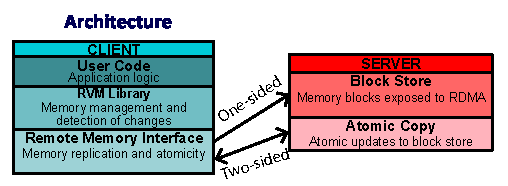
\includegraphics{lasagna.pdf}
\end{frame}

\begin{frame}{The RVM API}
    \begin{itemize}
        \item rvm\_cfg\_create() / rvm\_cfg\_destroy()
        \item rvm\_alloc() / rvm\_free()
        \item rvm\_txn\_start() / rvm\_txn\_commit()
        \item rvm\_set\_usr\_data() / rvm\_get\_usr\_data()
    \end{itemize}
\end{frame}

\begin{frame}{Two Backends}
    \begin{itemize}
        \item Infiniband RDMA
        \item RAMCloud
    \end{itemize}
\end{frame}

\begin{frame}{Backend API}
    \begin{itemize}
        \item put() / get()
        \item malloc() / free()
        \item atomic\_commit()
    \end{itemize}
\end{frame}

\begin{frame}{Infiniband Backend}
    \begin{itemize}
        \item put() and get() implemented using one-sided RDMA reads and writes
        \item other operations implemented using two-sided sends and receives
        \item atomicity achieved using shadow pages
        \item free() is transactional
    \end{itemize}
    \centering
    \includegraphics[scale=0.75]{ib-backend-arch.pdf}
\end{frame}

\begin{frame}{RAMCloud Backend}
    \centering
    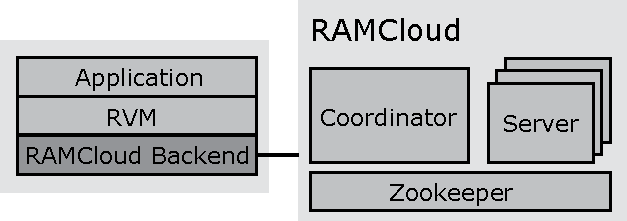
\includegraphics[scale=0.7]{ramcloud_backend_design_final.pdf}
    \vspace{2em}
    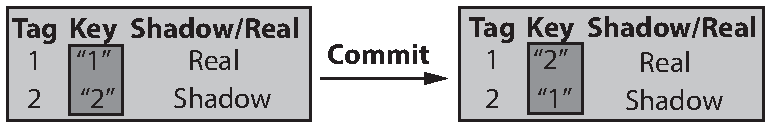
\includegraphics[scale=0.7]{ramcloud_backend_commit.pdf}
\end{frame}

\begin{frame}{Infiniband Microbenchmarks}
    \centering
    \begin{minipage}{0.45\textwidth}
        \centering
        Commit Latency

        \includegraphics[scale=0.25]{commit-results-rm.pdf}
    \end{minipage}
    \begin{minipage}{0.45\textwidth}
        \centering
        Recovery Latency

        \includegraphics[scale=0.25]{recovery-results-rm.pdf}
    \end{minipage}
\end{frame}

\begin{frame}{Infiniband Microbenchmarks}
    \centering
    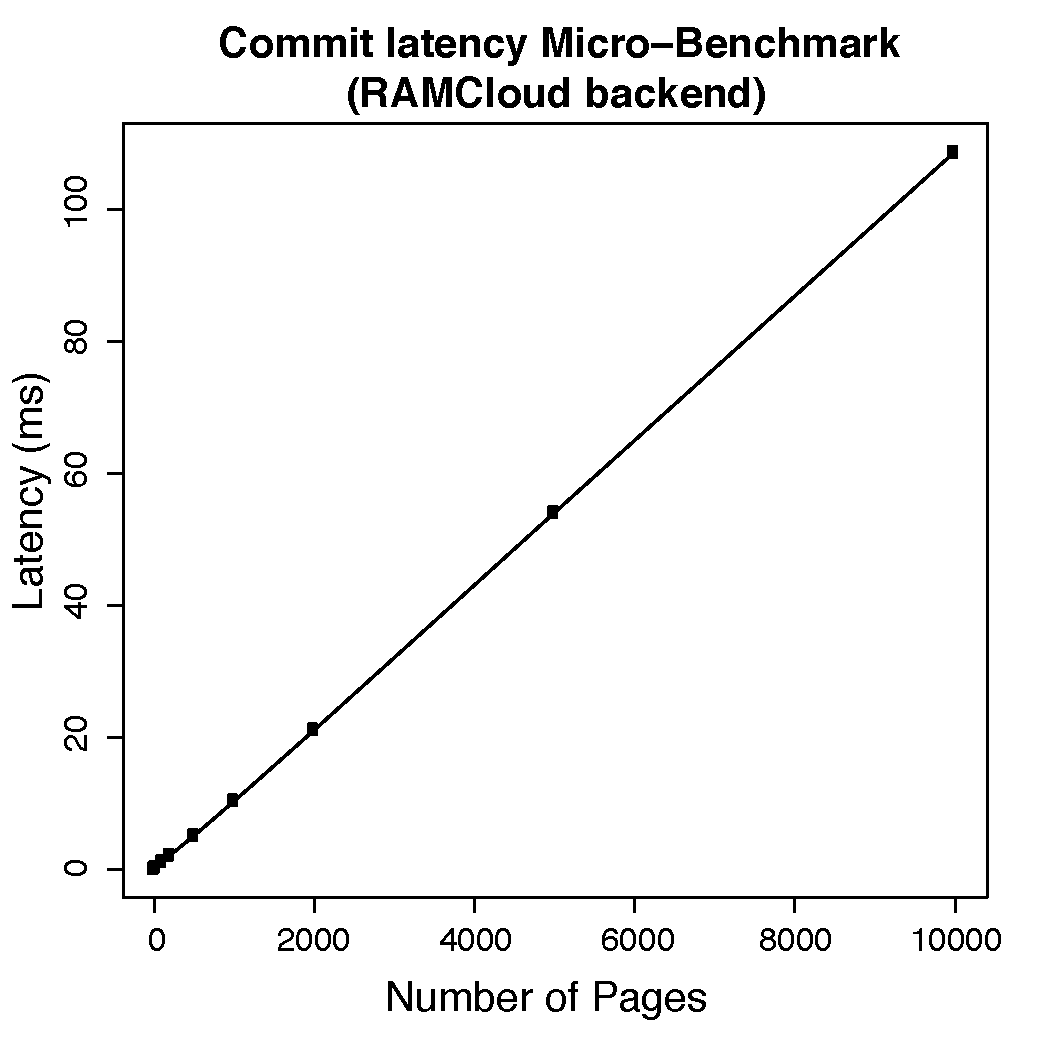
\includegraphics[scale=0.25]{commit_time_rc_latencies.pdf}
    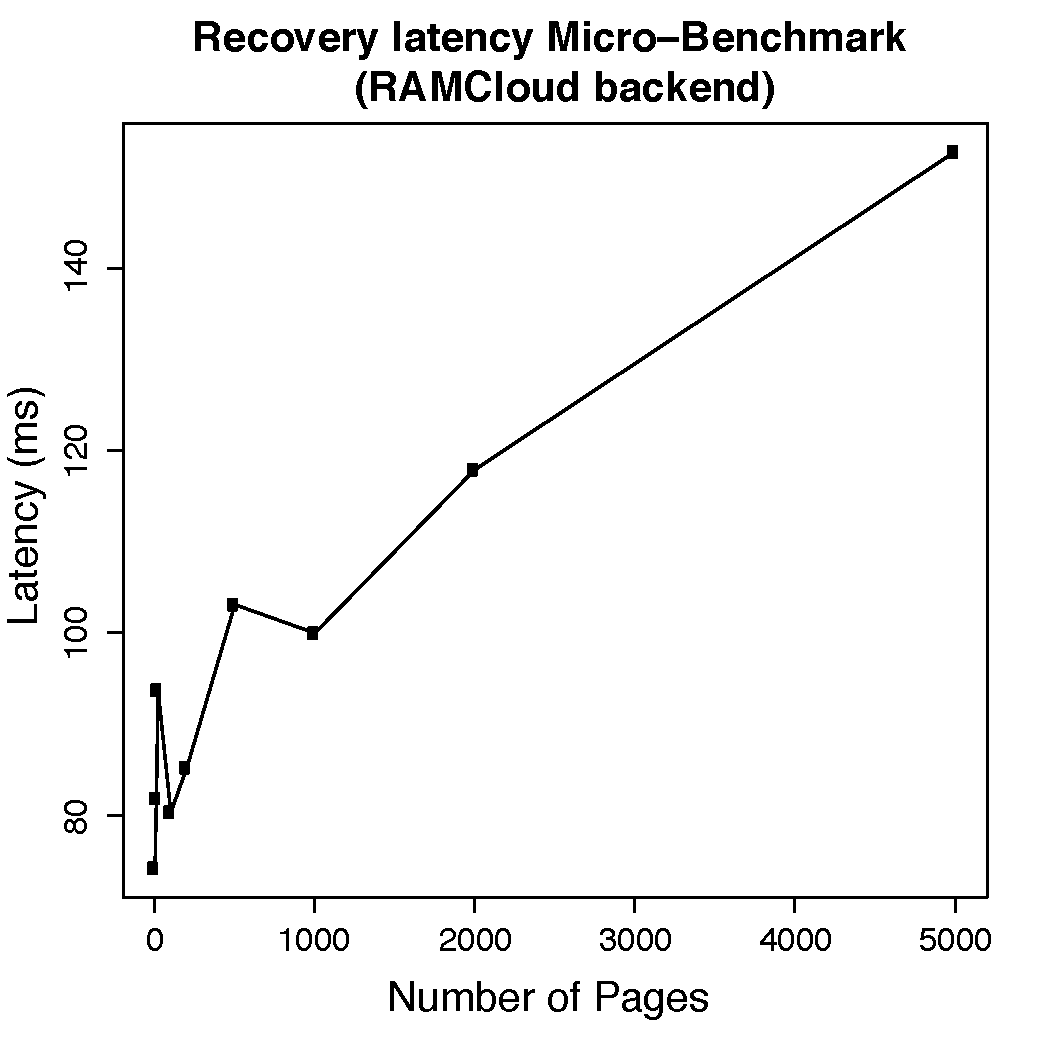
\includegraphics[scale=0.25]{recovery_time_rc_latencies.pdf}
\end{frame}

\begin{frame}{BLCR Microbenchmarks}
    \centering
    \begin{minipage}{0.45\textwidth}
        \centering
        Commit Latency

        \includegraphics[scale=0.25]{commit-results-blcr.pdf}
    \end{minipage}
    \begin{minipage}{0.45\textwidth}
        \centering
        Recovery Latency

        \includegraphics[scale=0.25]{recovery-results-blcr.pdf}
    \end{minipage}
\end{frame}

\begin{frame}{DGEMV Benchmark}
    \centering
    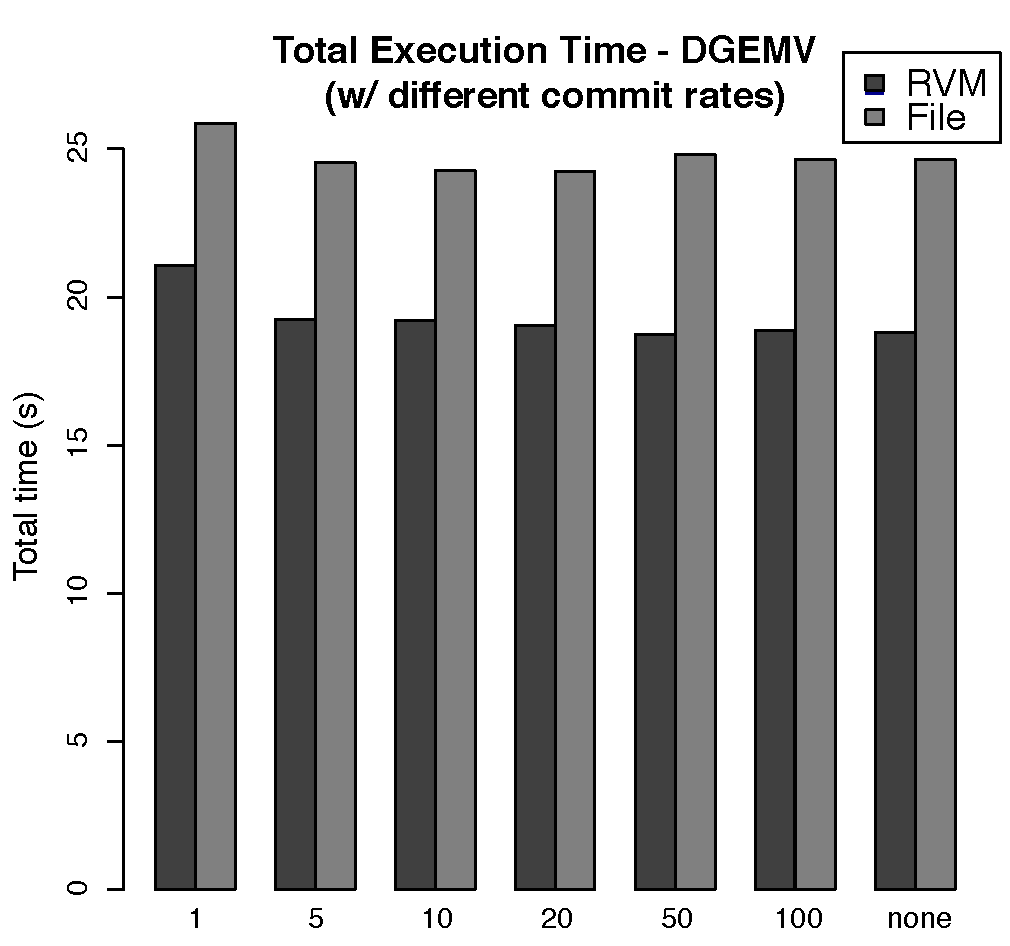
\includegraphics[scale=0.25]{dgemv_total_time_commit.pdf}
    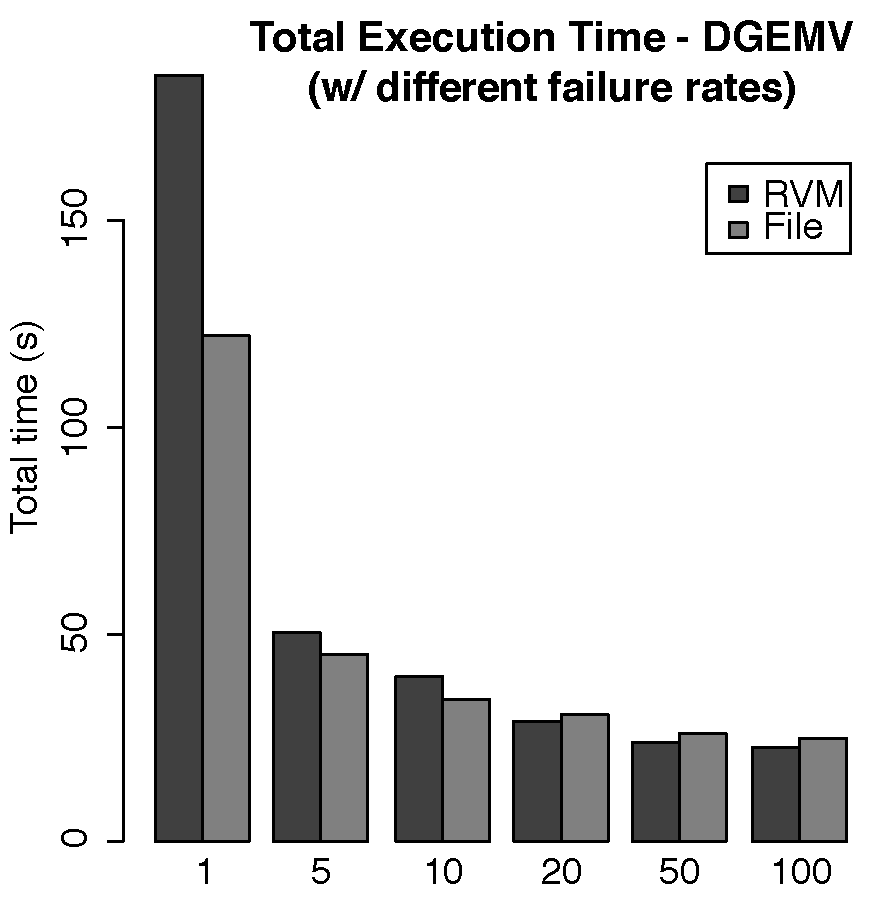
\includegraphics[scale=0.25]{dgemv_total_time_fail.pdf}
\end{frame}

\begin{frame}{Gene Assembly Benchmark}
    \centering
    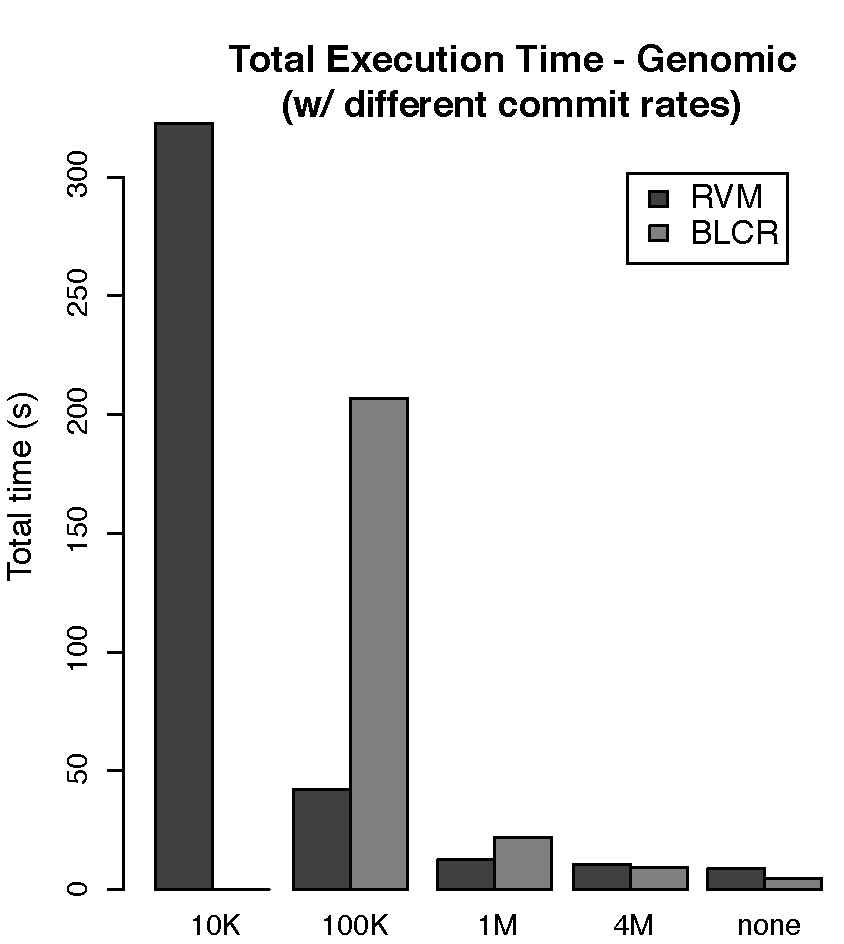
\includegraphics[scale=0.25]{genome_total_time_commit.pdf}
\end{frame}

\begin{frame}{Future Work}
    \begin{itemize}
        \item Improve performance
        \item Explore alternative backends
        \item Explore different consistency semantics
    \end{itemize}
\end{frame}

\begin{frame}{Custom RDMA Controller}
    \begin{itemize}
        \item Prototype of Firebox RDMA controller on FPGA
        \item Simpler API than Infiniband
        \item Remove need for page table pinning
    \end{itemize}
\end{frame}

\end{document}
